\chapter{Grundlagen}
Im ersten Teil dieses Kapitels werden die theoretischen Grundlagen, welche in den folgenden Kapitel dieser Arbeit Verwendung finden, erläutert. Als erstes erfolgt eine kurze Einführung in maschinelles Lernen mit Neuronalen Netzen und Deep Learning. Danach wird eine spezielle Form dieser Netzwerke vorgestellt, das sogenannte \emph{Convolutional Neural Network}, im folgenden \gls{cnn} genannt. Zuletzt wird noch kurz auf das sogenannte \emph{Distant Supervision} \cite{go2009twitter} eingegangen und dieses in Kontext mit der gegebenen Fragestellung (vgl. \ref{introduction}) gesetzt.\\\\
Im zweiten Teil wird auf die Anforderungen sowie die Implementation der Software zum Durchführen der Experimente eingegangen.

\section{Definitionen}
\subsection{Sentiment}
\blindtext
\subsection{Domäne / Crossdomain}
\blindtext
\section{Neuronale Netze}
\blindtext
\section{Deep Learning}
\blindtext
\section{Convolutional Neural Network}
\blindtext
\section{Word Embeddings}
\blindtext
\section{Distant-Phase Learning}
\blindtext
\section{Technische Implementation}
Im folgenden Abschnitt wird der technische Aufbau, welcher verwendet wurde, um die in \ref{experiments} beschriebenen Experimente durchzuführen.

\subsubsection{Vorarbeiten}
\label{technichal_setup:prework}
Der Grundaufbau der verwendeten Software wurde von Jan Deriu mithilfe von Keras\footnote{https://keras.io/} implementiert und zur Durchführung dieser Arbeit zur Verfügung gestellt. Im Rahmen dieses Grundaufbaus wurde die folgende Funktionalität bereits implementiert:

\begin{itemize}[noitemsep]
	\item Implementation des CNN in Keras und verwendung von Theano \cite{theanoCitShort} als Backend für die GPUs (vgl. Abschnitt \ref{technichal_setup:hardware}).
	\item Implementation von Evaluations-Metriken
	\item Skripte mit den folgenden Funktionalitäten: Trainieren des CNN, Laden von TSV Dateien, Vorverarbeiten von Word-Embeddings
\end{itemize}

\subsubsection{Anforderungen}
\label{technical_setup:requirements}
Ein System, welches die in \ref{experiments} beschriebenen Experimente durchzuführen, soll folgende Eigenschaften aufweisen:

\begin{itemize}
	\item \textbf{Parametrisierbarkeit}: Dadurch dass eine grosse Anzahl kleiner Experimente durchgeführt werden muss soll das System die Möglichkeit bitten Experimente parametrisiert durchzuführen.
	\item \textbf{Wiederholbarkeit}: Experimente sollen wenn nötig mehrfach durchgeführt werden ohne einen Mehraufwand zu verursachen. 
	\item \textbf{Übersichtlichkeit}: Resultate der Experimente sollen übersichtlich und einfach zugänglich sein.
	\item \textbf{Auswertbarkeit}: Resultate sollen \fixme{Bessers Wort für Einfach?} einfach ausgewertet werden können.
\end{itemize}

Die in \ref{technichal_setup:prework} beschriebenen Vorarbeiten bitten eine Basis um damit ein System aufzubauen, welche die oben beschriebenen Eigenschaften aufweist.
\subsubsection{Funktionalität}
\label{technical_setup:functionality}
Um ein System, welches die im vorhergehenden Kapitel beschriebenen Eigenschaften aufweist, zu erhalten, wurden die folgenden Komponenten implementiert:

\begin{itemize}
	\item \textbf{Executor}: Der \emph{Executor} ist zuständig für das Training der CNNs mithilfe von Keras. Beim Start akzeptiert er die Konfiguration als Parameter. Das Experiment wird mit dem Laden der benötigten Daten und dem anschliessenden Trainings des CNN gestartet. Am Ende jeder Epoche wird das aktuelle CNN auf den Validierungsdaten getestet und die konfigurierten Metriken ausgewertet. Diese werden am Ende zusammen mit dem trainierten CNN (Gewichte im HDF5-Format\footnote{https://support.hdfgroup.org/HDF5/}, das CNN Model als JSON) in einen für das Experiment vorgesehenen Ordner gespeichert. Die Metriken werden ebenfalls in diesem dem dafür vorgesehenen Ordner abgespeichert.
	\item \textbf{Config Management}: Experimente werden über Konfigurationen im JSON-Format\footnote{http://www.json.org/} parametrisiert. Über diese Konfiguration können viele wichtige Parameter für die Ausführung festgelegt werden, so zum Beispiel: Anzahl Epochen, Trainings- und Validierungsdaten, Parameter für k-fold Cross-Validation oder auch bereits Trainierte Modelle können geladen werden. Für eine vollständige Liste wird auf den Quellcode des Projektes verwiesen. Experimente können mitte§ls der group{\_}id gruppiert werden. Damit können die Experimente hierarchisch mittels zwei Ebenen gruppiert werden.
	\item \textbf{DataLoader}: Mithilfe des \emph{DataLoader} können Trainings- und Validierungsdaten im TSV\footnote{https://reference.wolfram.com/language/ref/format/TSV.html} Dateiformat geladen werden. Die zu ladenden Daten können dabei aus einer oder mehreren TSV-Dateien stammen.
\end{itemize}
\fixme{Referenze auf Code, Code-Style bei group{\_}id}
Die oben beschriebenen Komponenten erlauben es Experimente mittels JSON Konfigurationen zu starten und den gesamten Trainings- und Validierungsprozess mittels 

\subsubsection{Skripte}
Für die Durchführung der Experimente wurden diverse Skripte erstellt um die Handhabung zu vereinfachen und Auswertungen zu ermöglichen. Die Liste der implementierten Script umfasst unter anderem die folgenden:

\begin{itemize}[noitemsep]
	\item Erstellen von Plots der Lernkurven und Metriken
	\item Erstellen von Word-Embeddings über einen Textcorpus
	\item Erstellen von Statistiken zu Trainings- und Validierungsdaten
	\item Vorverarbeitung von Trainingsdaten für die Distant-Phase
	\item Erstellen von Visualisierungen von Word-Embeddings mittels t-SNE \cite{maaten2008visualizing}.
	\item Diverse Wartungsscripkte zur Generierung und Verwaltung von Experimenten
\end{itemize}

\subsubsection{Weboberfläche}
Um die dritte Anforderung nach Übersichtlichkeit und Auswertbarkeit (vgl. \ref{technical_setup:requirements}) zu erfüllen wurde eine Weboberfläche umgesetzt, mit welchem die Parameter und Resultate aller durchgeführten Experimente übersichtlich und an einem Ort zur Verfügung gestellt werden. Für die Implementation wurde das Python Framework flask\footnote{http://flask.pocoo.org/} verwendet.\fixme{Bilder der Weboberfläche, Schrift flask}\\
Zur Auswertung der Experimente stehen drei Funktionen zur Verfügung:
\begin{itemize}
	\item Die Oberfläche gewährt Zugriff auf alle JSON Konfigurationen, welche zu einem Experiment gehören. Dazu zählen die Konfiguration selbst, die gespeicherten Trainings- und Validierungsmetriken und das CNN Model (vgl. \ref{technical_setup:functionality}).
	\item Mittels der Plotting Funktion können Plots von Trainingsmetriken erstellt werden. Weiterhin können Plots und Boxplots über die die Validierungsmetriken der einzelnen Schritte der Crossdomain-Experimente (vgl. \ref{methods:v8}) erstellt werden.
	\item Die gespeicherten Validierungs- und Trainingsmetriken können mithilfe von math.js\footnote{http://mathjs.org/} direkt im Browser ausgewertet werden.\fixme{Code-Style}
\end{itemize}
\begin{figure}[htbp]
	\centering
	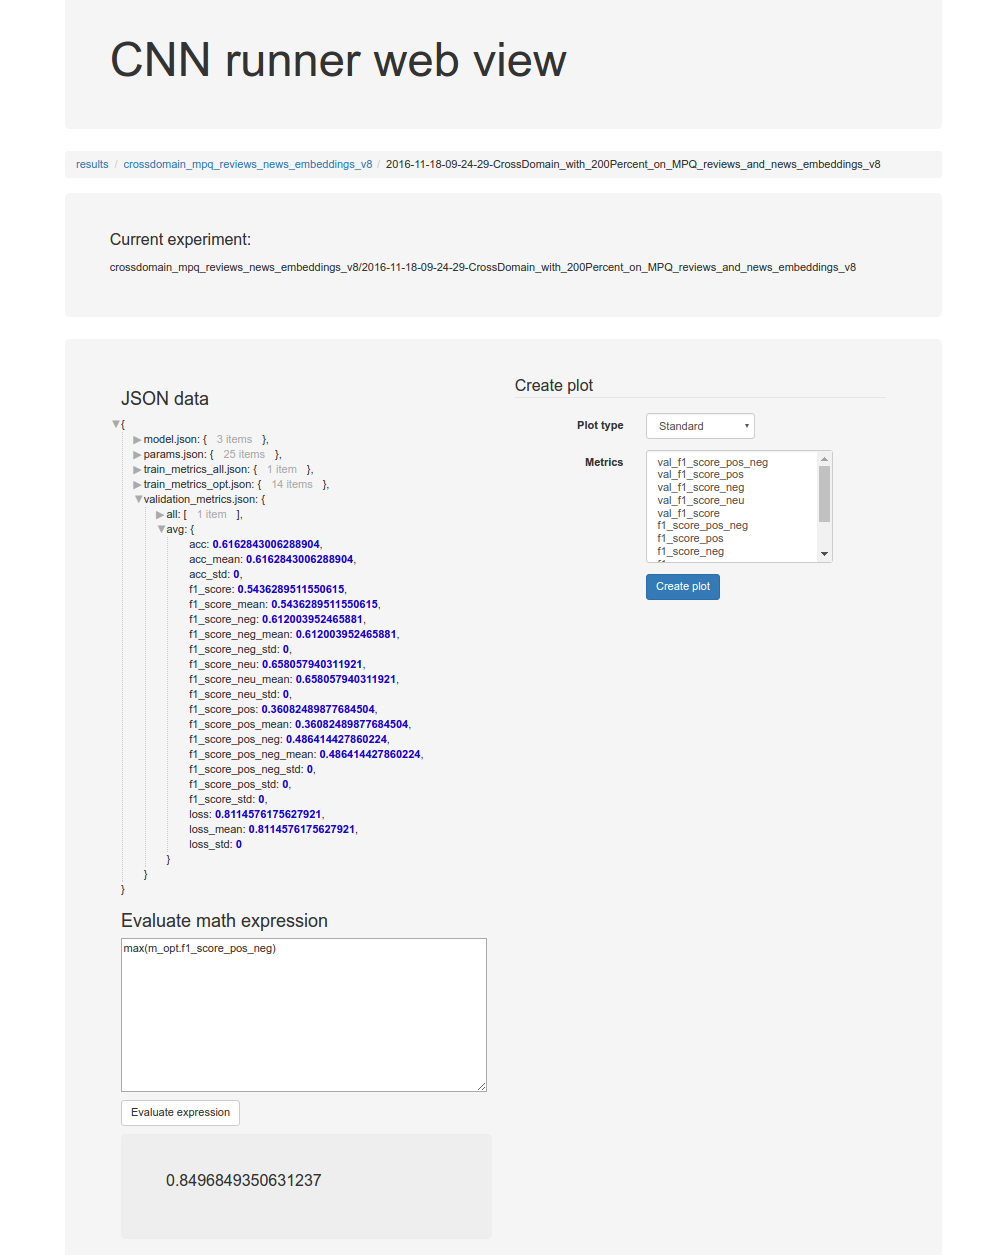
\includegraphics[width=0.7\textwidth]{img/web_gui}
	\caption{Ansicht Experiment über Weboberfläche}
	\label{fig:web_gui}
\end{figure}
\subsubsection{Betriebssystem \& Softwarepakete}
\label{technical_setup:software}
Alle Experimente wurden mit der unten beschriebenen Implementation durchgeführt. Auf beiden verwendeten Computer-Systemen (vgl. \ref{technichal_setup:prework}) wurde als Betriebssystem Ubuntu 16.04 installiert. Dazu wurden Python 3.5.2\footnote{https://www.python.org/}, Nvidia GPU Treiber und cuda8\footnote{https://developer.nvidia.com/cuda-toolkit} als Abhängigkeiten von Theano und Keras installiert.

\subsection{Hardware}
\label{technichal_setup:hardware}
Zur Durchführung der Experimente wurden zwei unterschiedliche Computer verwendet. Im ersten System (S1) ist eine Nvidia GTX970 GPU, einen Intel i7 4950K CPU und 16GB Arbeitsspeicher installiert. Das zweite System besitzt eine Nvidia GTX1070 GPU, einen Intel i7 6700K CPU und ebenfalls 16GB Arbeitsspeicher. Die Unterschiede in der Hardware haben keinen Einfluss auf die Experimente, da auf beiden System dasselbe Betriebssystem mit den gleichen Softwarepaketen verwendet wurde (vgl. \ref{technical_setup:software}).

